\documentclass[]{article}
\usepackage[margin=0.5in]{geometry}
\usepackage{amsthm}
\usepackage{mathtools}
\usepackage{amsfonts}
\usepackage{tikz}
\usetikzlibrary{matrix}

\newtheorem{definition}{Definition}[section]
\newtheorem{theorem}{Theorem}[section]
\newtheorem{lemma}[theorem]{Lemma}



%opening
\title{Verifying Featured Transition Systems using Variability Parity Games}
\author{Sjef van Loo}

\begin{document}

\maketitle

\section{Introduction}
Model verification techniques can be used to improve the quality of software. These techniques require the behaviour of the software to be modelled, after which the model can checked to verify that it behaves conforming to some requirement. Different languages are proposed and well studied to express these requirements, examples are LTL, CTL, CTL* and $\mu$-calculus (TODO: cite). Once the behaviour is modelled and the requirement is expressed in some language we can use modal checking techniques to determine if the model satisfies the requirement.

These techniques are well suited to model and verify the behaviour of a single software product. However software systems can be designed to have certain parts enabled or disabled. This gives rise to many software products that all behave very similar but not identical, such a collection is often called a \textit{product family}. The differences between the products in a product family is called the \textit{variability} of the family. A family can be verified by using the above mentioned techniques to verify every single product independently. However this approach does not use the similarities in behaviour of these different products, an approach that would make use of the similarities could potentially be a lot more efficient.

\textit{Labelled transition systems} (LTSs) are often used to model the behaviour of a system, while it can model behaviour well it cannot model variability. Efforts to also model variability include I/O automata, modal transition systems and \textit{featured transition systems} (FTSs) (TODO: cite). Specifically the latter is well suited to model all the different behaviours of the software products as well as the variability of the entire system in a single model.

Efforts have been made to verify requirements for entire FTSs, as well as to be able to reason about features. Notable contributions are fLTL, fCTL and fNuSMV (TODO: cite). However, as far as we know, there is no technique to verify an FTS against a $\mu$-calculus formula. Since the modal $\mu$-calculus is very expressive, it subsumes other temporal logics like LTL, CTL and CTL*, this is desired. In this thesis we will introduce a technique to do this. We first look at LTSs, the modal $\mu$-calculus and FTSs. Next we will look at an existing technique to verify an LTS, namely solving \textit{parity games}, as well as show how this technique can be used to verify an FTS by verifying every software product it describes independently. An extension to this technique is then proposed, namely solving \textit{variability parity games}. We will formally define variability parity games and prove that solving them can be used to verify FTSs.

\section{Definitions}
\subsection{Transition systems}
Similar to \cite{Classen2013FeaturedTS}.

\begin{definition}
	\label{def_lts}An LTS is a tuple $M = (S, Act, trans, s_0)$, where:
	\begin{itemize}
		\item $S$ is a set of states,
		\item $Act$ a set of actions,
		\item $trans \subseteq S \times Act \times S$ is the transition relation with $(s,a,s') \in trans$ denoted by $s \xrightarrow a s'$,
		\item $s_0 \in S$ is the initial state.
	\end{itemize}
\end{definition}

\begin{definition}
	\label{def_fts}An FTS is a tuple $M = (S, Act, trans, s_0, N, P, \gamma)$, where:
	\begin{itemize}
		\item $S, Act, trans, s_0$ are defined as in an LTS,
		\item $N$ is a non-empty set of features,
		\item $P \subseteq \mathcal{P}(N)$ is a set of products, ie. feature assignments, that are valid,
		\item $\gamma : trans \rightarrow \mathbb{B}(N)$ is a total function, labelling each transition with a Boolean expression over the features. A product $p \in \mathcal{P}(N)$ satisfying the Boolean expression of transition $t$ is denoted by $p \models \gamma(t)$, $\gamma(t)(p) = 1$ or $p \in [\![\gamma(t)]\!]$. 
		
		A transition $s \xrightarrow a s'$ and $\gamma((s,a,s')) = f$ is denoted by $s \xrightarrow {a / f} s'$. 
	\end{itemize}
\end{definition}

\begin{definition}
	\label{def_fts_proj}
	The projection of an FTS $M$ to a product $p \in P$, noted $M_{|p}$, is the LTS $M'=(S,Act,trans', s_0)$, where $trans' = \{t \in trans\ |\ p \models \gamma(t)\}$.
\end{definition}

\begin{definition}
	\label{def_mu_syntax}\cite{Groote}
	A modal $\mu$-calculus formula over the set of actions $Act$ and a set of variables $\mathcal{X}$ is defined by
	\[ \varphi = \top\ |\ \bot\ |\ X\ |\ \varphi \vee \varphi\ |\ \varphi \wedge \varphi\ |\ \langle a \rangle \varphi\ |\ [a]\varphi\ |\ \mu X.\varphi\ |\ \nu X.\varphi \]
	with $a \in Act$ and $X \in \mathcal{X}$. 
	
	
	No negations in the language because negations can be pushed inside to the propositions, ie. the $\top$ and $\bot$ elements.
\end{definition}
A fixed point formula $ \sigma X. \varphi$, with $\sigma \in \{\mu,\nu\}$, can be unfolded which results in the formula $\varphi$ where very $X$ is replaced by $\sigma X. \varphi$, ie. $\varphi[X:=\sigma X. \varphi]$. A fixed point formula is equivalent to its unfolding, ie. $\sigma X. \varphi$ is equivalent to $\varphi[X:=\sigma X. \varphi]$. \cite{Bradfield2018}

\begin{definition} 
	\label{def_mu_sem}\cite{Groote} For LTS $(S, Act, trans, s_0)$ we inductively define the interpretation of a modal $\mu$-calculus formula $\varphi$, notation
	$[\![ \varphi ]\!]^\rho$, where $\rho : \mathcal{X} \rightarrow \mathcal{P}(S)$ is a logical variable valuation, as a set of states
	where $\varphi$ is valid, by:
	\begin{align*}
	&[\![ \mathit{\top} ]\!]^\rho &&= S\\
	&[\![ \mathit{\bot} ]\!]^\rho &&= \emptyset\\
	&[\![ \varphi_1 \wedge \varphi_2 ]\!]^\rho &&= [\![ \varphi_1 ]\!]^\rho \cap [\![ \varphi_2 ]\!]^\rho \\
	&[\![ \varphi_1 \vee \varphi_2 ]\!]^\rho &&= [\![ \varphi_1 ]\!]^\rho \cup [\![ \varphi_2 ]\!]^\rho\\
	&[\![ \langle a \rangle \varphi ]\!]^\rho &&= \{s \in S|\exists_{s' \in S} s \xrightarrow {a} s' \wedge s' \in [\![ \varphi ]\!]^\rho\}\\
	&[\![ [ a ] \varphi ]\!]^\rho &&= \{s \in S|\forall_{s' \in S} s \xrightarrow {a} s' \implies s' \in [\![ \varphi ]\!]^\rho\}\\
	&[\![ \mu X. \varphi ]\!]^\rho &&= \bigcap_{f \subseteq S}\{f | f = [\![ \varphi ]\!]^{\rho[X:=f]}\}\\
	&[\![ \nu X. \varphi ]\!]^\rho &&= \bigcup_{f \subseteq S}\{f | f = [\![ \varphi ]\!]^{\rho[X:=f]}\}\\
	&[\![ X ]\!]^\rho &&= \rho(X)
	\end{align*}
\end{definition}
\begin{definition}
	\label{def_sat}
	Given LTS $M = (S, Act, trans, s_0)$, state $s \in S$ and mu-calculus formula $\varphi$ we write $M,s \models \varphi$ if and only if $\varphi$ is satisfied in state $s$ for LTS $M$. If $M, s_0 \models \varphi$ we write $M \models \varphi$.
\end{definition}
\section{Goal}
Similar to \cite{inproceedings}.

Given an FTS $M = (S, Act, trans, s_0, N, P, \gamma)$ and a modal $\mu$-calculus formula $\varphi$ we want to find the set $P_s \subseteq P$ such that:
\begin{itemize}
	\item for every $p \in P_s$ we have $M_{|p} \models \varphi$,
	\item for every $p \in P \backslash P_s$ we have $M_{|p} \not\models \varphi$.
\end{itemize}
A counterexample for every $p \in P \backslash P_s$ is preferred.

If $P_s = P$, ie. all products satisfy $\varphi$, we write $M \models \varphi$.

\section{Parity Games}
\subsection{Parity games}
\begin{definition}
	\label{def_PG}\cite{Bradfield2018}
	A parity game (PG) is a tuple $(V, V_0, V_1, E, \rho)$, where:
	\begin{itemize}
		\item $V = V_0 \cup V_1$ and $V_0 \cap V_1 = \emptyset$,
		\item $V_0$ is the set of vertices owned by player $0$,
		\item $V_1$ is the set of vertices owned by player $1$, 
		\item $E \subseteq V \times V$ is the edge relation,
		\item $\rho :  V \rightarrow \mathbb{N}$ is a priority assignment.
	\end{itemize}
\end{definition}
We write $\alpha \in \{0,1\}$ to denote an arbitrary player. We write $\overline{\alpha}$ to denote $\alpha$'s opponent, ie. $\overline{0} = 1$ and $\overline{1} = 0$.

A parity game is played by players 0 and 1. A play starts with placing a token on vertex $v \in V$. Player $\alpha$ moves the token if the token is on a vertex owned by $\alpha$, ie. $v \in V_\alpha$. The token can be moved to $w \in V$, with $(v,w) \in E$. A series of moves results in a sequence of vertices, called path. For path $\pi$ we write $\pi_i$ to denote the $i^{\text{th}}$ vertex in path $\pi$. A play ends when the token is on vertex $v \in V_\alpha$ and $\alpha$ can't move the token anywhere, in this case player $\overline{\alpha}$ wins the play. If the play results in an infinite path $\pi$ then we determine the highest priority that occurs infinitely often in this path, formally
\[ \max\{ p \ |\ \forall_j \exists_i j < i \wedge p = \rho(\pi_i) \}\] 
If the highest priority is odd then player $1$ wins, if it is even player $0$ wins.

A strategy for player $\alpha$ is a function $\sigma : V^*V_\alpha \rightarrow V$ that maps a path ending in a vertex owned by player $\alpha$ to the next vertex. Parity games are positionally determined \cite{Bradfield2018}, therefore a strategy $\sigma: V_\alpha \rightarrow V$ that maps the current vertex to the next vertex is sufficient. 

A strategy $\sigma$ for player $\alpha$ is winning from vertex $v$ if and only if any play that results from following $\sigma$ results in a win for player $\alpha$. The graph can be divided in two partitions $W_0 \subseteq V$ and $W_1 \subseteq V$, called winning sets. If and only if $v \in W_\alpha$ then player $\alpha$ has a winnings strategy from $v$. Every vertex in the graph is either in $W_0$ or $W_1$ \cite{Bradfield2018}. Furthermore finite parity games are decidable \cite{Bradfield2018}.
\subsection{Featured parity games}
\begin{definition}
	\label{def_FPG}
	A featured parity game (FPG) is a tuple $(V,V_0, V_1, E, \rho, N, P, \gamma)$, where:
	\begin{itemize}
		\item $V = V_0 \cup V_1$ and $V_0 \cap V_1 = \emptyset$,
		\item $V_0$ is the set of vertices owned by player $0$,
		\item $V_1$ is the set of vertices owned by player $1$, 
		\item $E \subseteq V \times V$ is the edge relation,
		\item $\rho :  V \rightarrow \mathbb{N}$ is a priority assignment,
		\item $N$ is a set of features,
		\item $P \subseteq \mathcal{P}(N)$ is a set of products, ie. feature assignments, for which the game can be played,
		\item $\gamma : E \rightarrow \mathbb{B}(N)$ is a total function, labelling each edge with a Boolean expression over the features.
	\end{itemize}
\end{definition}
An FPG is played similarly to a PG, however the game is played for a specific product $p \in P$. Player $\alpha$ can only move the token from $v \in V_\alpha$ to $w \in V$ if $(v,w) \in E$ and $p \models \gamma(v,w)$.

A game played for product $p \in P$ results in winnings sets $W_0^p$ and $W_1^p$, which are defined similar to the $W_0$ and $W_1$ winning sets for parity games.

\begin{definition}
	\label{def_FPG_proj}
The projection from FPG $G = (V,V_0, V_1, E, \rho, N, P, \gamma)$ to a product $p \in P$, noted $G_{|p}$, is the parity game $(V,V_0,V_1, E', \rho)$ where $E' = \{ e \in E\ |\ p \models \gamma(e) \}$.
\end{definition}

Playing FPG $G$ for a specific product $p\in P$ is the same as playing the PG $G_{|p}$. Any path that is valid in $G$ for $p$ is also valid in $G_{|p}$ and vice versa. Therefore the strategies are also interchangeable, furthermore the winning sets $W_\alpha$ for $G_{|p}$ and $W_\alpha^p$ for $G$ are identical. Since parity games are positionally determined so are FPGs. Similarly, since finite parity games are decidable, so are finite FPGs.

\subsection{Variability parity games}
\begin{definition}
	\label{def_VPG}
	A variability parity game (VPG) is a tuple $(V,V_0, V_1, E, \rho, \mathfrak{C}, \theta)$, where:
	\begin{itemize}
		\item $V = V_0 \cup V_1$ and $V_0 \cap V_1 = \emptyset$,
		\item $V_0$ is the set of vertices owned by player $0$,
		\item $V_1$ is the set of vertices owned by player $1$, 
		\item $E \subseteq V \times V$ is the edge relation; we assume that $E$ is total, i.e. for all $v\in V$ there is some $w \in V$ such that $(v,w) \in E$,
		\item $\rho :  V \rightarrow \mathbb{N}$ is a priority assignment,
		\item $\mathfrak{C}$ is a finite set of configurations,
		\item $\theta : E \rightarrow \mathcal{P}(\mathfrak{C})\ \backslash\ \{0\}$ is the configuration mapping, satisfying for all $v \in V$, $\bigcup\{\theta(v,w)|(v,w) \in E\} = \mathfrak{C}$.
	\end{itemize}
\end{definition}
A VPG is played similarly to a PG, however the game is played for a specific configuration $c \in \mathfrak{C}$. Player $\alpha$ can only move the token from $v \in V_\alpha$ to $w \in V$ if $(v,w) \in E$ and $c \in \theta(v,w)$. Furthermore VPGs don't have deadlocks, every play results in an infinite path.

A game played for configuration $c \in \mathfrak{C}$ results in winning sets $W_0^c$ and $W_1^c$, which are defined similar to the $W_0$ and $W_1$ winning sets for parity games.

\begin{definition}
	\label{def_VPG_proj} The projection from VPG $G = (V, V_0, V_1, E, \rho, \mathfrak{C}, \theta)$ to a configuration $c \in \mathfrak{C}$, noted $G_{|c}$, is the parity game $(V, V_0, V_1, E', \rho)$ where $E' = \{ e\in E | c \in \theta(e)\}$.
\end{definition}

Playing VPG $G$ for a specific configuration $c \in \mathfrak{C}$ is the same as playing the PG $G_{|c}$. Any path that is valid in $G$ for $c$ is also valid in $G_{|c}$ and vice versa. Therefore the strategies are also interchangeable, furthermore the winning sets $W_\alpha$ for $G_{|c}$ and $W_\alpha^c$ for $G$ are identical. Since parity games are positionally determined so are VPGs. Similarly, since finite parity games are decidable, so are finite VPGs.

\subsection{Creating parity games}
Originating from an FTS and a modal $\mu$-calculus we can create an FPG (from which we can create a PG by projection) and from the FPG we can create a VPG. For a specific product we can project the FTS to an LTS, from which we can create a PG. The relation between the transition systems and games is displayed in the following diagram.
\\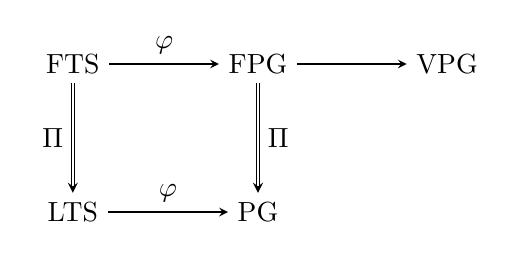
\begin{tikzpicture}
\matrix (m) [matrix of math nodes,row sep=4em,column sep=4em,minimum width=2em]
{
	\text{FTS} & \text{FPG} & \text{VPG} \\
	\text{LTS} & \text{PG} \\};
\path[-stealth]
(m-1-1) edge [double] node [left] {$\Pi$} (m-2-1)
edge node [above] {$\varphi$} (m-1-2)
(m-2-1.east|-m-2-2) edge node [above] {$\varphi$}
 (m-2-2)
(m-1-2) edge [double] node [right] {$\Pi$} (m-2-2)
edge (m-1-3);
\end{tikzpicture}\\
The projections are defined in the previous section. In this section we will define the horizontal arrows in the diagram. First we show how to create a PG from an LTS and a  modal $\mu$-calculus formula, this part is well studied and the approach is based on \cite{Bradfield2018}.


\begin{definition}
	\label{def_LTS2PG}\cite{Bradfield2018}
	LTS2PG($M, \varphi$) converts LTS $M = (S, Act, trans, s_0)$ and closed formula $\varphi$ to a PG $(V, V_0, V_1, E, \rho)$.
	
	A vertex in the parity game is represented by a pair $(s, \psi)$ where $s \in S$ and $\psi$ is a modal $\mu$-calculus formula. We will create a vertex for every state with every subformula of $\varphi$ except subformula's of the form $X$. Furthermore we create a vertex for every state with the unfolding of every fixpoint formula. Formally we define the set of vertices by first defining the set of subformula's:
	\[ F = \{ \psi\ |\ \psi \text{ is a subformula of } \varphi \} \text{, note that $\varphi$ is a subformula of $\varphi$} \]
	The set of subformula's that are of the form $X$:
	\[ F_X = \{ \psi \in F\ |\ \psi = X\} \]
	 And the set of the unfolding of fixedpoint subformula's:
	 \[ F_\sigma = \{\psi[X:=\sigma X. \psi]\ |\ \sigma X. \psi \in F \text{ with } \sigma \in \{\mu, \nu\}\} \]
	Having these sets we can define the set of vertices by:
	\[ V = S \times (F \backslash F_X \cup F_{\sigma})\]
	
	We create the parity game with the smallest set $E$ such that:
	\begin{itemize}
		\item $V = V_0 \cup V_1$,
		\item $V_0 \cap V_1 = \emptyset$ and
		\item for every $v = (s, \psi) \in V$ we have:
		\begin{itemize}
			\item If $\psi = \top$ then $v \in V_1$.
			\item If $\psi = \bot$ then $v \in V_0$.
			\item If $\psi = \psi_1 \vee \psi_2$ then:
				\subitem $v \in V_0$,
				\subitem $(v, (s,\psi_1)) \in E$ and
				\subitem $(v, (s,\psi_2)) \in E$.
			\item If $\psi = \psi_1 \wedge \psi_2$ then:
				\subitem $v \in V_1$,
				\subitem $(v, (s,\psi_1)) \in E$ and
				\subitem $(v, (s,\psi_2)) \in E$.
			\item If $\psi = \langle a \rangle \psi_1$ then $v \in V_0$ and for every $s \xrightarrow{ a} s'$ we have $(v, (s', \psi_1)) \in E$.
			\item If $\psi = [ a ] \psi_1$ then $v \in V_1$ and for every $s \xrightarrow{ a} s'$ we have  $(v, (s', \psi_1)) \in E$.
			\item If $\psi = \mu X. \psi_1$ then $(v, (s, \psi_1[X:=\mu X. \psi_1])) \in E$.
			\item If $\psi = \nu X. \psi_1$ then $(v, (s, \psi_1[X:=\nu X. \psi_1])) \in E$.
		\end{itemize}
	Note that since $\varphi$ is closed and we use unfolding there will never be an edge $(v,(s, X)) \in E$.
	\end{itemize}


Finally we have $\rho(s, \psi) = \begin{cases}
2 \lfloor adepth(X) / 2 \rfloor & \text{if } \psi = \nu X. \psi'\\
2 \lfloor adepth(X) / 2 \rfloor + 1 & \text{if } \psi = \mu X. \psi'\\
0 & \text{otherwise}
\end{cases}$
\end{definition}
Next we define the transformation from FTS to FPG.
\begin{definition}
	\label{def_FTS2FPG}
	FTS2FPG($M, \varphi$) converts FTS $M = (S, Act, trans, s_0, N, P, \gamma)$ and closed formula $\varphi$ to FPG $(V, V_0, V_1, E, \rho, N, P, \gamma')$.
	
	We have $(V, V_0, V_1, E, \rho)$ = LTS2PG($(S, Act, trans, s_0), \varphi$) and
	\[ \gamma'((s, \psi),(s', \psi')) = \begin{cases}
	\gamma(s,a,s') & \text{if }\psi = \langle a \rangle \psi'\text{ or }\psi = [a]\psi' \\
	\top & \text{otherwise}
	\end{cases}\]
\end{definition}
Finally we define how to create a VPG from an FPG. This transformation abstracts from the notion of products and uses configurations for a syntactically more pleasant representation. Furthermore in VPGs deadlocks are removed, this is done by creating two losing vertices $l_0$ and $l_1$ such that player $\alpha$ loses when the token is in vertex $l_\alpha$. Any vertex that can not move for a configuration will get an edge that is admissible for that configuration towards one of the losing vertices.
\begin{definition}
	\label{def_FPG2VPG}
	FPG2VPG($G^F$) converts FPG $G^F = (V^F, V_0^F, V_1^F, E^F, \rho^F, N, P, \gamma)$ to VPG $G = (V, V_0, V_1, E, \rho, \mathfrak{C}, \theta)$.
	
	Let $P$ be defined as  $\{p_0, p_1, \dots, p_m\}$, we define $\mathfrak{C} = \{c_0, c_1, \dots, c_m\}$.
	
	We create vertices $l_0$ and $l_1$ and define $V_0 = V_0^F \cup \{l_0\}$, $V_1 = V_1^F \cup \{l_1\}$ and $V = V_0 \cup V_1$.
	
	We construct $E$ by first making $E = E^F$ and adding edges $(l_0, l_0)$ and $(l_1, l_1)$ to $E$. Simultaneously we construct $\theta$ by first making $\theta(e) = \{c_i \in \mathfrak{C} | p_i \models \gamma(e)\}$ for every $e \in E^F$. Furthermore $\theta(l_0,l_0) = \theta(l_1,l_1) = \mathfrak{C}$.
	
	Next, for every vertex $v \in V_\alpha$ with $\alpha = \{0,1\}$, we have $C = \mathfrak{C} \backslash \bigcup \{\theta(v,w)|(v,w) \in E\}$. If $C \neq \emptyset$ then we add $(v, l_\alpha)$ to $E$ and make $\theta(v,l_\alpha) = C$.
	Finally we have 
	\[ \rho(v) = \begin{cases}
	1  & \text{if } v = l_0 \\
	0 & \text{if } v = l_1 \\
	\rho^F(v) &\text{otherwise}
	\end{cases} \]
\end{definition}

\subsection{Correctness}
\begin{theorem}
	\label{the_PGsubPGA} Given:
	\begin{itemize}
		\item FTS $M = (S,Act, trans, s_0, N, P, \gamma)$,
		\item a closed modal mu-calculus formula $\varphi$,
		\item a product $p \in P$
	\end{itemize}
	it holds that he parity games LTS2PG($M_{|p}, \varphi$) and FTS2FPG($M, \varphi$)$_{|p}$  are identical.
\begin{proof}
	Let $G^F = $FTS2FPG($M, \varphi$)$ = (V^F, V_0^F, V_1^F, E^F, \rho^F, N, P, \gamma')$, using definition \ref{def_FTS2FPG}, and $G^F_{|p} = (V^F, V_0^F, V_1^F, {E^F}', \rho^F)$, using definition \ref{def_FPG_proj}. Furthermore we have $M_{|p} = (S, Act, trans', s_0)$ and we let $G = $ LTS2PG$(M_{|p}, \varphi) = (V, V_0, V_1, E, \rho)$. We depict the different transition systems and games in the following diagram.
	
	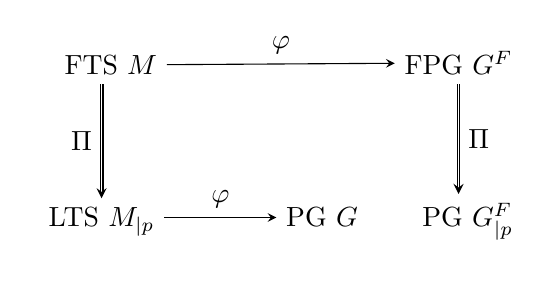
\begin{tikzpicture}
	\matrix (m) [matrix of math nodes,row sep=4em,column sep=1em,minimum width=2em]
	{
		\text{\ \ FTS }M & \  &\ & \text{FPG } G^F  \\
		\text{LTS }M_{|p} & \ & \text{PG } G & \text{\ \ PG }G_{|p}^F \\};
	\path[-stealth]
	(m-1-1) edge [double] node [left] {$\Pi$} (m-2-1)
	edge node [above] {$\varphi$} (m-1-4)
	(m-2-1.east|-m-2-3) edge node [above] {$\varphi$}
	(m-2-3)
	(m-1-4) edge [double] node [right] {$\Pi$} (m-2-4);
	\end{tikzpicture}\\
	We will prove that $G = G_{|p}^F$. We first note that game $G$ is created by 
	\[  (V, V_0, V_1, E, \rho) = LTS2PG((S, Act, trans', s_0),\varphi) \]
	and the vertices, edges and priorities of game $G^F$ are created by 
	\[ (V^F, V_0^F, V_1^F, E^F, \rho^F) = LTS2PG((S,Act, trans, s_0), \varphi)\]
	Using the definition of LTS2PG (\ref{def_LTS2PG}) we find that the vertices and the priorities only depend on the states in $S$ and the formula $\varphi$, since these are identical in the above two statements we immediately get $V = V^F, V_0 = V_0^F, V_1 = V_1^F$ and $\rho = \rho^F$. The vertices and priorities don't change when an FTS is projected, therefore $G_{|p}^F$ has the same vertices and priorities as $G^F$.
	
	Now we are left with showing that $E = {E^F}'$ in order to conclude that that $G = G^F_{|p}$. We will do this by showing $E \subseteq {E^F}'$ and $E \supseteq {E^F}'$.
	
	First let $e \in E$. Note that a vertex in the parity game is represented by a pair of a state and a formula. So we can write $e = ((s,\psi),(s',\psi'))$. To show that $e \in {E^F}'$ we distinguish two cases:
	\begin{itemize}
		\item  If $\psi = \langle a \rangle \psi_1$ or $\psi = [a] \psi_1$ then there exists an $a \in Act$ such that $(s,a,s') \in trans'$. Using definition \ref{def_fts_proj} we get $(s,a,s') \in trans$ and $p \models \gamma(s,a,s')$. Using definition \ref{def_FTS2FPG} we find that $\gamma'((s,\psi),(s',\psi')) = \gamma(s,a,s')$ and therefore $p \models \gamma'((s,\psi),(s',\psi'))$. Now using definition \ref{def_FPG_proj} we find $((s,\psi),(s',\psi')) \in {E^F}'$.
		\item Otherwise the existence of the edge does not depend on the $trans$ parameter and therefore $((s,\psi),(s',\psi')) \in {E^F}'$ if $(s,\psi) \in V^F$, since $V^F = V$ we have $(s,\psi) \in V^F$.
	\end{itemize}
	We can conclude that $E \subseteq {E^F}'$, next we will show $E \supseteq {E^F}'$. Let $e = ((s,\psi),(s',\psi')) \in {E^F}'$. We distinguish two cases:
	\begin{itemize}
		\item If $\psi = \langle a \rangle \psi_1$ or $\psi = [a] \psi_1$ then there exists an $a \in Act$ such that $(s,a,s') \in trans$. Using definition \ref{def_FPG_proj} we get $p \models \gamma'(s,a,s')$. Using definition \ref{def_FTS2FPG} we get $p \models \gamma(s,a,s')$. Using the projection definition \ref{def_FTS2FPG} we get $(s,a,s') \in trans'$ and therefore $((s,\psi),(s',\psi'))\in E$.
		\item Otherwise the existence of the edge does not depend on the $trans$ parameter and therefore $((s,\psi),(s',\psi')) \in E$ if $(s,\psi) \in V$, since $V^F = V$ we have $(s,\psi) \in V$.
	\end{itemize}
	\end{proof}
\end{theorem}

\begin{theorem}
	\label{the_FPG_ver_FTS}
	Given:
	\begin{itemize}
		\item FTS $M = (S, Act, trans, s_0, N, P, \gamma)$,
		\item closed modal mu-calculus formula $\varphi$,
		\item product $p \in P$ and
		\item state $s \in S$
	\end{itemize}
it holds that $M_{|p}, s \models \varphi$ if and only if $(s, \varphi) \in W_0^p$ in FTS2FPG($M, \varphi$).
\begin{proof}
	The winning set $W_\alpha^p$ is equal to winning set $W_\alpha$ in FTS2FPG($M, \varphi$)$_{|p}$ using definition \ref{def_FPG}. Using theorem \ref{the_PGsubPGA} we find that the game FTS2FPG($M, \varphi$)$_{|p}$ is equal to the game LTS2PG($M_{|p}, \varphi$), obviously their winning sets are also equal. Using the modal verification proof from \cite{Bradfield2018} we know that $M_{|p}, s \models \varphi$ if and only if $(s, \varphi) \in W_0$. Winning set $W_\alpha^p$ is equal to $W_\alpha$, therefore the theorem holds.
\end{proof}
\end{theorem}

\begin{theorem}
	\label{the_FPG_sub_VPG}
	Given:
	\begin{itemize}
		\item FPG $G^F = (V^F, V_0^F, V_1^F, E^F, \rho^F, N, \{p_0, p_1, \dots, p_m\}, \gamma)$,
		\item product $p_i$,
		\item player $\alpha \in \{0,1\}$
	\end{itemize}
we have for winning sets $W_\alpha^{p_i}$ in $G$ and $W_\alpha^{c_i}$ in FPG2VPG($G^F$) that $W_\alpha^{p_i} \subseteq W_\alpha^{c_i}$.
\begin{proof}
	Let $G = (V,V_0,V_1, E, \rho, \mathfrak{C},\theta) =$ FPG2VPG($G^F$). Consider finite play $\pi$ that is valid in game $G^F$ for product $p_i$. We have for every $(\pi_i, \pi_{i+1})$ in $\pi$ that $(\pi_i, \pi_{i+1}) \in E^F$ and $p_i \models \gamma((\pi_i, \pi_{i+1}))$. From definition \ref{def_FPG2VPG} it follows that $(\pi_i, \pi_{i+1}) \in E$ and $c_i \in \theta(\pi_i, \pi_{i+1})$. So we can conclude that path $\pi$ is also valid in game $G$ for configuration $c_i$. Since the play is finite the winner is determined by the last vertex $v$ in $\pi$, player $\alpha$ wins such that $v \in V_{\overline{\alpha}}$. Furthermore we know, because the play is finite, that there exists no $(v,w) \in E^F$ with $p \models \gamma(v,w)$. From this we can conclude that $(v, l_{\overline{\alpha}}) \in E$ and $c_i \in \theta(v, l_{\overline{\alpha}})$. Vertex $l_{\overline{\alpha}}$ has one outgoing edge, namely to itself. So finite play $\pi$ will in game $G^F$ results in an infinite play $\pi(l_{\overline{\alpha}})^\omega$. Vertex $l_{\overline{\alpha}}$ has a priority with the same parity as player $\alpha$, so player $\alpha$ wins the infinite play in $G$ for configuration $c_i$.
	
	Consider infinite play $\pi$ that is valid in game $G^F$ for product $p_i$. As shown above this play is also valid in game $G$ for configuration $c_i$. Since the win conditions of both games are the same the play will result in the same winner.
	
	Consider infinite play $\pi$ that is valid in game $G$ for configuration $c_i$. We distinguish two cases:
	\begin{itemize}
		\item If $l_\alpha$ doesn't occur in $\pi$ then the path is also valid for game $G^F$ with product $p_i$ and has the same winner.
		\item If $\pi = \pi'(l_\alpha)^\omega$ then the winner is player $\overline{\alpha}$. The path $\pi'$ is valid for game $G^F$ with product $p_i$. Let vertex $v$ be the last vertex of $\pi'$. Since $(v, l_\alpha) \in E$ and $c_i \in \theta(v,l_\alpha)$ we know that there is no $(v,w) \in E^F$ with $p_i \models \gamma(v,w)$ and that vertex $v$ is owned by player $\alpha$. So in game $G^F$ player $\alpha$ can't move at vertex $v$ and therefore loses the game (in which case the winner is also $\overline{\alpha}$.
	\end{itemize}

We have shown that every path (finite or infinite) in game $G^F$ with product $p_i$ can be played in game $G$ with configuration $c_i$ and that they have the same winner. Furthermore every infinite path in game $G$ with configuration $c_i$ can be either played as an infinite path or the first part of the path can be played in $G^F$ with product $p_i$ and they have the same winner. From this we can conclude that the theorem holds.
\end{proof}
\end{theorem}
\bibliography{mybib} 
\bibliographystyle{ieeetr}

\end{document}
